\documentclass[letterpaper,11pt]{report}
\usepackage[boxed]{algorithm2e}
\usepackage{algpseudocode}
\usepackage{fullpage}
\usepackage{verbatim}
\usepackage{cite}
\usepackage{setspace}
\usepackage{fancyhdr}
\usepackage{amsmath}


%\usepackage{noReferences}
\usepackage[small]{caption}
\usepackage[leftcaption]{sidecap}
\usepackage{graphics}
\usepackage{color}

\usepackage{hyperref}

%\usepackage{natbib}

\usepackage[dvips]{graphicx}
 % define the title
\graphicspath{ {images/}}

% Paper conservation layout. Long live the trees!!
\setlength{\oddsidemargin}{-0.4mm} % 25 mm left margin
\setlength{\evensidemargin}{\oddsidemargin}
\setlength{\textwidth}{160mm}      % 25 mm right margin
\setlength{\topmargin}{-5.4mm}     % 20 mm top margin
\setlength{\headheight}{5mm}
\setlength{\headsep}{5mm}
\setlength{\footskip}{10mm}
\setlength{\textheight}{237mm}     % 20 mm bottom margin


\setlength{\parskip}{1ex}
\parindent 0in
\def\SAONE{Specific Aim 1}
\def\SATWO{Specific Aim 2}
\def\SATHREE{Specific Aim 3}
\def\SAFOUR{Specific Aim 4}

\def\title{Mytitle}
%\def\titletwo{Thesis Proposal Title Line 2}

\begin{document}





\def\addrone{Your address}
\def\addrtwo{Your city}

\def\degree{M.Tech. in Computer Science with Specialization in Data Engineering}


\def\submissiondate{June 01, 2014}

\def\supervisorone{Haimonti Dutta}

\def\supervisortwo{Srikanta Bedathur}

\def\supervisorthree{Lipika Dey}


%\def\supervisorfour{XXX XXXX }


%\def\supervisorfive{YYY YYYY}

\thispagestyle{empty}

\begin{center}

{\LARGE \bf {FINDING INFLUENTIAL PEOPLE FROM A HISTORICAL NEWS REPOSITORY }

 }  
 \vspace{.3in}
 
 {\Large{Student Name: Aayushee Gupta}} \\  
 \vspace{.1in} 
 IIIT-D-MTech-CS-DE-12-030 \\

% Nov 30, 2011 \\
  
    \vspace{.35in}

  \vspace{.25in}

{Indraprastha Institute of Information Technology\\
New Delhi}

\vspace{.35in}  {\underline{Thesis Committee} \\ \supervisorone         
   \\ \supervisortwo \\ \supervisorthree }\\ \vspace{.35in}


 {Submitted in partial fulfillment of the requirements \\for the Degree of M.Tech. in Computer Science, \\ with specialization in Data Engineering}

\vspace{.2in}

\copyright 2014 SSSSSS SSSSSS \\ All rights reserved \\
\vspace{.8in}


\end{center}


\newpage

\pagestyle{empty}
\vspace*{7.1in} 
Keywords: Gazetteer, Text Mining, Information Retrieval, OCR, Spelling Correction, Historical data 

\newpage

\begin{center}
\section*{Certificate}\label{section:certificate}
\end{center}
%\vspace{3in}
This is to certify that the thesis titled \textbf{``Title Title Title Title Title Title Title Title Title Title Title Title"} submitted by \textbf{Student Name} for the partial fulfillment of the requirements for the degree of \emph{Master of Technology} in \emph{Computer Science \& Engineering} is a record of the bonafide work carried out by her / him under my / our guidance and supervision in the Security and Privacy group at Indraprastha Institute of Information Technology, Delhi. This work has not been submitted anywhere else for the reward of any other degree. \\ \vspace{0.5in}

\textbf{Professor Advisor Name}\\
\textbf{Indraprastha Institute of Information Technology, New Delhi}
%\doublespacing

\begin{abstract}


Historical archives of newspapers provide a wealth of information which can be used for a variety of purposes. They are of interest to genealogists, historians and scholars for efficiently searching articles pertaining to people in a chronological fashion. 
A people gazetteer can be defined as a list of chain of articles related to a person entity occurring in a news article over a historical timeline.

In this thesis we present the process of construction of a people
gazetteer from noisy OCR text and the novel problem of finding
influential people from it. To build the people gazetteer we first
spell correct the noisy text using an edit distance algorithm. A novel
N-gram evaluation algorithm is used for measuring its performance.
We construct the people gazetteer by collecting occurrences of person entities using Named Entity Recognition and linking them with a chain of articles that he/she is related to.
The chain of articles for each person entity is created by finding similarity among news articles based on LDA topic detection model.
We then define an Influential Person Index based on each person entity's chains of articles and rank them as influential across various newspaper topics based on this index.  
Our corpus is a sample of 14020 newspaper articles obtained from Chronicling America project undertaken by the Library of Congress.

\end{abstract}

\newpage
\pagestyle{empty}


\newpage



\section*{Acknowledgments}\label{section:acknowledgments}
\pagestyle{plain}
\pagenumbering{roman}

XXXXXX XXXXXX XXXXXX XXXXXX XXXXXX XXXXXX XXXXXX XXXXXX XXXXXX XXXXXX XXXXXX XXXXXX XXXXXX XXXXXX XXXXXX XXXXXX XXXXXX XXXXXX XXXXXX XXXXXX XXXXXX XXXXXX XXXXXX XXXXXX XXXXXX XXXXXX XXXXXX XXXXXX XXXXXX XXXXXX XXXXXX XXXXXX 

\newpage

\tableofcontents
\listoffigures 
\listoftables

\newpage

\newpage

\newpage
\mbox{}


%\doublespacing

\chapter{Introduction}\label{chapter:introduction}
%\pagestyle{fancy}
\pagenumbering{arabic}
\setcounter{page}{1}
\onehalfspacing

Aim?

Motivation? 

What is a Gazetteer?

Gate Gazetteer
The goal of this research is to enable users to find influential people in a gazetteer of historical newspaper archives. The main users  include genealogists and other library patrons so that  they can efficiently search for articles relating to people that are of interest to them across several newspaper categories on a timeline.


\chapter{Related Work}
\chapter{Data Preprocessing}\label{chapter:data preprocessing} 

 
This chapter describes the dataset used for research purpose and the preprocessing steps that are performed to minimize the garbled text in it.
 
\section{Data}

The dataset for research is taken from Chronicling America \footnote{http://chroniclingamerica.loc.gov/} website which provides 100 years of historical newspaper scanned images as well as their raw OCR text without any punctuation marks. The OCR text provided is on a page by page level and no article level segmentation is provided. So the OCR text dataset is taken from the PostgreSQL database of CCLS servers where article level segmentation has been done for two months of articles of "The Sun" newspaper from November-December 1894 consisting of 14020 news articles. The individual text articles generated from the database do not have any punctuation and contain a large amount of garbled text with several types of errors. An individual OCR text article has at least one or more of the following types of errors:

\begin{figure}[hbt]
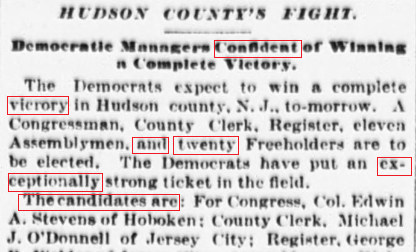
\includegraphics[scale=0.75]{originalimage}
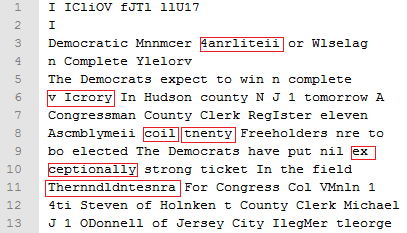
\includegraphics[scale=0.80]{ocr}
\caption{Scanned Image of a Newspaper article (left) and its OCR raw text (right)}
\end{figure}

\begin{description}
 \item[$\bullet$Real word errors] include words that are spelled correctly in the OCR text but still incorrect when compared to the original newspaper article image. For example: In Figure 3.1, the word "coil"  has been correctly spelled in the OCR text  but should have been "and" according to the original newspaper article. 
 \item[$\bullet$Non-real word errors] include words that have been misspelled due to some insertion, deletion, substitution or transposition of characters from a word. For eg. In Figure 3.1, the word "tnenty" in the OCR text has a substitution error ('n' should have been 'w') which is actually "twenty" according to the original newspaper article.
 \item[$\bullet$Non-word errors] include words that have been spelled incorrectly and are a combination of alphabets and numerical characters. For example: In Figure 3.1, the word "4anrliteii" which is a combination of alphabets and number and should have been "confident" as per the original newspaper article.
\item[$\bullet$New Line errors] include words that are separated by hyphens where part of a word is written on one text line and remaining part in the next line. For example: In Figure 3.1, the word "ex-ceptionally" where "ex" occurs on one line while "ceptionally" in the next and due to no punctuation in the text, they are treated as separate words in OCR text.
\item[$\bullet$Word Break and Join errors] include words that either get broken down into one of more parts or some words in a sentence get joined to a make a single word. For example: In Figure 3.1, the word "Thernndldntesnra" in the OCR text is actually a combination of three words "The candidates are" while the words "v Icrory" are actually equivalent to a single word "victory" when compared with the original news article.
\end{description} 

OCR errors exist in huge numbers in the dataset making it extremely garbled and difficult to work with. The text needs to be preprocessed in some manner in order to be used for any text mining task. Following section describes the preprocessing of OCR dataset.

\section{Spelling Correction}
 The garbled OCR text consists of several kinds of spelling errors and needs to be refined by correcting the text with the help of a spelling corrector. The main aim of the research being finding influential people, so the spelling correction of person named entities must also be given due consideration so that the person names entities with correct spellings get detected as a result.
The following sections describe the spelling correction algorithm as well as its testing and evaluation results on the OCR dataset.

\subsection{Related Work}
//BRIEF REVIEW OF PAPERS REGARDING SPELLING CORRECTION OF OCR DATA

\subsection{Spelling Correction Algorithm}

The spelling correction algorithm used works on isolated word correction using dictionary based-look up method and distance between strings for matching the text and correcting it.
The Edit Distance algorithm based on Levenshtein distance\cite{levenshtein1966binary} has been used to correct the spellings. An "edit distance" corresponds to the minimum number of insertions, deletions, and substitutions required to transform one string into another. The algorithm corrects Non-Real Word spelling errors up to an edit distance of 2 , i.e. , it corrects words which have spelling errors that can be corrected by making at most 2 operations of insertion, deletion and substitution of letters in the word.
The spelling corrector has been designed as suggested by Peter Norvig \footnote{ http://norvig.com/spell-correct.html}. The algorithm requires a dictionary which is used to check if each word of the text exists in it or not. If the word already exists in the dictionary then no change is made to the word and if not, then a candidate list of words is created from the word to be corrected by inserting, substituting or deleting up to 2 letters from it. This list of words is again checked for in the dictionary and returned as suggestions for the word to be corrected. The correction is made with the word formed from lowest edit distance and occurring with more frequency in the dictionary. This makes the edit distance algorithm dependent on the type of dictionary chosen for correction which means the dictionary must be well chosen for spelling correction of a specific document collection. The algorithm runs faster by reading the dictionary only once and keeping a data structure in memory for its word counts which can be referred to whenever a word comes up for correction.

\subsection{Spelling Correction Algorithm Evaluation}
Following sections describe the evaluation parameters for estimating the performance of Spelling Corrector on the OCR dataset:

\subsubsection{Accuracy}

To test the performance of this algorithm, the raw OCR text and OCR text after application of spelling correction algorithm needs to be compared with the original newspaper text. The OCR text is extremely garbled with Word Break and Join errors due to which word-to-word alignment with the original newspaper text is impossible. For this purpose, a testing algorithm has been developed for evaluation. The evaluation metric used for measuring the performance of Spelling correction algorithm is Accuracy which requires calculation of how many OCR errors got corrected when compared to the original scanned newspaper text. The measure has been chosen so as to include the complete text coverage and not just check for words that got corrected after spell correction as in the latter case, the  number of FP and TN get missed which won't give the correct measure of how well the spell corrector works. The formula used for calculating Accuracy is defined by Manning and Schutze,1999 (p.268-269) as follows:

$Accuracy=  \dfrac{TP+FP} {TP+ FP + TN + FN}$


where 

TP=Number of True Positives,

TN=Number of True Negatives,

 FP=Number of False Positives,

 FN=Number of False Negatives. 

The aim of the testing algorithm is to make a word-to-word correspondence between the OCR corrected text and the original OCR text and to mark each token in the OCR text as a TP, FP, TN or FN. Reynaert and Martin\cite{reynaert2008all} suggest a way to define these terms by distinguishing between correct words and incorrect words in the text through the set of non-target, target and selected words.  

According to our spelling corrector, a "true positive" is said to occur when a word from the OCR text gets corrected and the corrected spelling matches the one in original article text while a "false positive" occurs if the corrected spelling does not match the corresponding word in the original article text. A "true negative" occurs when a word does not get corrected by the algorithm as it is already correct and matches the correct word in the original text also. On the other hand, a "false negative" occurs when the algorithm is unable to correct the word (there is no change in spelling of the word) and it does not match the corresponding word in the original text but should have been corrected.

To make this correspondence, a window of n-word grams in the scanned image text article is considered (Original.txt). For each token in the spell corrected text (Corrected.txt), the corresponding token  in the scanned text article along with 2 tokens before and 2 tokens after it are considered for alignment. If the token being considered matches with any of these words in the scanned text article words window and its spelling has been corrected when compared to the corresponding token in raw OCR text (OCR.txt), then it is marked as a "True Positive" which is actually rewarding the Spell corrector for making the correct spelling change. A "False Positive" is marked if it does not match any of the words despite its spelling being corrected. If the token being considered matches any of the words in the words window but no spelling correction has been made for it, then it is marked as a "True Negative" and if it does not match any word in the window and the spelling corrector also did not correct it, then it is marked as a "False Negative" as the word got missed by the corrector. 

Several cases could occur like difference in the lengths of linetext between OCR and Original text or while considering the first, second or the last tokens from the Corrected text for which the corresponding word window in Original text needs to be smaller. All such cases have been covered in the algorithm which calls function 'MatchWordGrams' for these different cases. 

A limitation of this evaluation algorithm is that it requires all 3 versions of a newspaper article (Original, Corrected and OCR) to have the same number of lines. In case of difference in the number of lines of text due to some Word Break and Join errors, the words window needs to be extended so as to cover previous and next line texts also for alignment.


\begin{algorithm}[!h]
\caption{Evaluation Algorithm for Spell Correction}
  \KwIn{Ocr.txt,Corrected.txt,Original.txt}
  \KwOut{Spell Corrector Accuracy }
\SetKwFunction{MatchWordGrams}{MatchWordGrams}%
 $OcrLine$:=a line of text from Ocr.txt\;
 $CorrectedLine$:=a line of text from Corrected.txt\;
 $OriginalLine$:=a line of text from Original.txt\;
 $tp \leftarrow $0  $fp \leftarrow $0 $tn \leftarrow $0 $fn\leftarrow $0\;  
	\For{(int i=0; i $<$ CorrectedLine.length ; i++) }
	{

    \If{(CorrectedLine.length$<$4 $||$ OriginalLine.length$<$4)}
	{		
    	\MatchWordGrams{(OcrLine,CorrectedLine,OriginalLine,0,OriginalLine.length,i)}\; 
	}
    \Else{
   \If {(i==0)}
   {
\MatchWordGrams{(OcrLine,CorrectedLine,OriginalLine,0,3,0)}\;
   }
   \ElseIf{ (i==1)}
   {
\MatchWordGrams{(OcrLine,CorrectedLine,OriginalLine,0,4,1)}\;
   }
	\ElseIf{(i==(CorrectedLine.length-2) $||$ (CorrectedLine.length-1) $||$ (CorrectedLine.length) $||$ (CorrectedLine.length+1))}
	{
\MatchWordGrams{(OcrLine,CorrectedLine,OriginalLine,i-2,OriginalLine.length,i)}\;
	}  
	\ElseIf{(i $>$= CorrectedLine.length+2)}
	{	
\MatchWordGrams{(OcrLine,CorrectedLine,OriginalLine,OriginalLine.length-3,OriginalLine.length,i)}\;	
	}
	\Else
	 {
\MatchWordGrams{(OcrLine,CorrectedLine,OriginalLine,i-2,i+2,i)}\;	
	}	
   }
 }
 	 $Accuracy=(tp+tn)/(tp+tn+fp+fn);$\
\end{algorithm}


\begin{algorithm}[!htb]
\caption{MatchWordGrams Function called by Algorithm 1}
\begin{algorithmic}
\Function {MatchWordGrams}{OcrLine, CorrectedLine, OriginalLine, jstart, jend, i}
  
 \For{(int j=jstart; j$<$jend; j++)}
  {
    \If{ ((CorrectedLine[i].equals(OriginalLine[j]))\&\&(!(OcrLine[i].equals(CorrectedLine[i]))))}
     {
	  $tp=tp+1$\;
	  flag0=false\;
	 \Return $tp$\;
	  }
	\ElseIf{((CorrectedLine[i].equals(OriginalLine[j]))\&\&(OcrLine[i].equals(CorrectedLine[i])))}
	      {
		 $tn=tn+1$\;
		  flag1=false\;
		\Return $tn$\;
	      }
}

	 \If{(!(OcrLine[i].equals(CorrectedLine[i]))\&\&flag0==true)}
	 {
		    $fp=fp+1$\;
		   \Return $fp$\;
            }
	 
	 \ElseIf{((OcrLine[i].equals(CorrectedLine[i])) \&\& flag1==true)}
	 {
		    $fn=fn+1$\;
		   \Return $fn$\;
	 }
\EndFunction
\end{algorithmic}
\end{algorithm}




\begin{figure} [!htb]
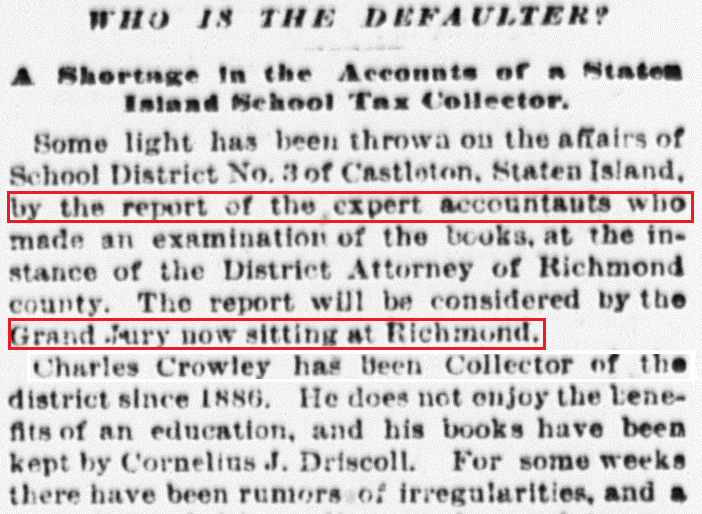
\includegraphics[scale=0.4]{img3}
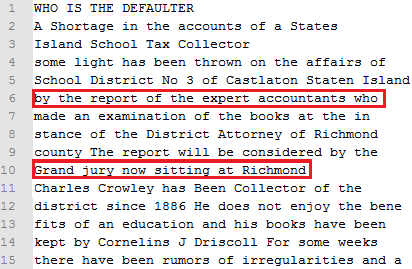
\includegraphics[scale=0.75]{originalimg3}
\caption{Scanned image of a newspape article (left) along with its original text (right)}
\end{figure}
 
\begin{figure}[h]
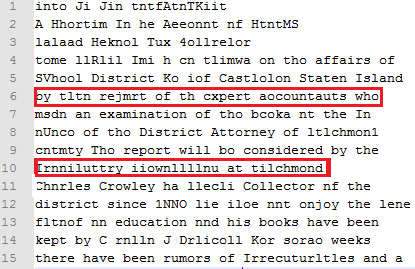
\includegraphics[scale=0.75]{ocr3}
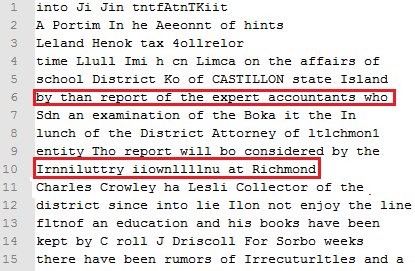
\includegraphics[scale=0.75]{corrected3}
\caption{OCR raw text (left) and Spell corrected text (right) of the article}
\end{figure}
\newpage Working of the above algorithm can be demonstrated with the help of the following example:
Consider 3 versions of a scanned image of a newspaper article,  the original text of the scanned image in Figure 3.2 and the raw OCR text and the corrected text (after spell correction) in Figure 3.3. As highlighted in the figures, for line 6 the line texts are:

\newpage OcrLine= \textit{by tltn rejmrt of th cepert aocountauts who}

CorrectedLine= \textit{by than report of the expert accountants who}

OriginalLine= \textit{by the report of the expert accountants who} 

Here, for each token of CorrectedLine, we find its index and call the MatchWordGrams function accordingly. For the first token 'by' at index i=0 in CorrectedLine, we consider the word window to be "by the report" (index j=0 to 2) in OriginalLine by matching iteratively with each token to see if there is a match and also if there has been a spelling correction by comparing with the corresponding token in OcrLine. Here, no change was made to the spelling of 'by' and it matches with a word in words window, so it is marked as a FN. For the second token 'than' at index i=1, we consider the word window to be "by the report of" (index j=0 to 3) for which there is no match in the window but there has been a spelling correction from 'tltn' to 'than', which implies the correction was wrong and the token is marked as a FP. For the third token 'report' at index i=2, we consider the window as "by the report of the" (index j=0 to 4) in Original Line and find that there is a match in the word window and there has been a spelling correction too from 'rejmrt' to 'report' which makes this token a TP. Similarly, rest of the tokens get marked for each line in the Corrected.txt. 

Another example can be considered from Line 10 in Figure 3.2 and Figure 3.3 where the number of tokens is different in CorrectedLine and OriginalLine. In such a case, direct alignment between tokens is not possible because of which the words window becomes useful. Here, when the last token 'Richmond' of CorrectedLine is considered at index i=3, the corresponding words window becomes "Jury now sitting at Richmond" (index j=1 to 5) for which there is a match in the words windows and corresponding spelling has also been changed from 'tilchmond' to 'Richmond' which makes it a TP. Had the word window not been considered, the corresponding token at index j=3 in OriginalLine would have been chosen as 'sitting' which would have resulted in a FP. 
   

\subsubsection{Time taken for Spelling Correction}
Time is also an essential parameter while measuring the performance of spelling correction. Since the dataset is quite large, it is important that the algorithm does not take too long to correct an article and can be parallelized in case it takes more time for correction.

\subsubsection{Person Names Detection Rate}
The spelling correction algorithm is evaluated on the basis of another parameter which is used to consider the special case of person entity names spelling correction as the main goal of research is to detect these names with correct spellings.
Person Names Detection Rate can be defined as the ratio of person names recognized through Named Entity Recognition before spelling correction process and the total number of person names recognized in the original newspaper articles.

$Person Names Detection Rate=\dfrac{ \text{Person Names recognized before/after spelling correction}} {\text{ Person Names recognized in original newspaper articles}} $


\subsection{Spelling Correction Algorithm Evaluation Results}
The spelling correction algorithm is used to correct all the 14020 OCR raw text articles in the dataset. The dictionary used for look-up is a concatenation of several public domain books from Project Gutenberg and lists of most frequent words from Wiktionary and the British National Corpus \footnote{http://norvig.com/big.txt} along with a large people names list which is obtained  by running Stanford NER-CRF parser on dataset from TREC 2013 Crowdsourcing track. \footnote{http://boston.lti.cs.cmu.edu/clueweb12/TRECcrowdsourcing2013/}
The spelling corrector is quite fast and takes 9 seconds on an average to correct the newspaper OCR articles. It takes a total of 36 hours to run on 14020 articles.
Though the algorithm does not require parallelizing here but it can be parallelized by getting candidate lists for insertion, deletion, substitution and transposition of a word through parallel threads and combining them together for correction of a word.
 
For evaluation of the spelling corrector, 3 versions of each newspaper article are required: OCR raw text, spelling corrector corrected text and the original scanned newspaper article text. Since the dataset is quite large (14020) and it is not possible to get original text of each of these newspaper images, a smaller number of articles are chosen to study the results of spelling correction. 50 scanned newspaper images are taken and an online OCR \footnote{www.onlineocr.net} is run on them followed by some manual correction to get the original articles text. 
Accuracy can then be calculated for all 3 versions of 50 newspaper articles using the Evaluation algorithm by marking each word in the OCR text article as a TP, FP, TN or FN. 

The spelling corrector shows an Accuracy of 72.7 \%  when corrected text is compared to OCR text and original article text. The results are less accurate due to a large number of Non-word, New Line, Word Join and Break errors in the OCR data which can not be corrected by the spelling correction algorithm.
But the spelling correction is useful in terms of PersonNamesDetectionRate \textit{(PNDR)}. Following are the statistics obtained for \textit{PNDR}:

\textit{PNDR} for Raw OCR Text: 72.5\% 

\textit{PNDR} for Spell Corrected Text without Person names correction: 63.3\% 

\textit{PNDR} for Spell Corrected Text after: 82.5\% 

These statistics indicate that spelling correction using an extended dictionary for personal names is useful for detecting person names from the garbled newspaper articles and the results are dependent on the type of dictionary being used for spell correction.
 
A better result can be obtained by correcting the New Line errors in the articles. This can be done by checking for if the word at last index of a text line or the word at first index of the next text line is a word not present in the dictionary and combining the two and checking again in the dictionary for a valid word. The new word, if present in the dictionary can be replaced by the two words from which it is formed thereby removing the New Line error. Similar approach can be applied for Word Break and Join errors but would require each word of an article not present in the dictionary to be analyzed along with some window of words before and after it to make a correction. 
 
\chapter{PEOPLE GAZETTEER}\label{chapter:people gazetteer}

This chapter describes the process of construction of people gazetter by extracting person names from the news articles dataset (NER) followed by formation of chains of articles for each person entity over different article topics using LDA topic detection.

Dataset statistics

Output of people gazetteer

\chapter{Influential People Detection}\label{chapter:influential people detection}
\chapter{Results and Conclusion}\label{chapter:results and conclusion}
%\newpage
%\bibliographystyle{these}
\bibliographystyle{acm}
%\bibliographystyle{elsart-harv}
%\newpage
%\section{References}
%\bibliography{Library}

\bibliography{aayushee}
\chapter*{Appendix}\label{chapter:appendix} 

\end{document}
